Deep learning is a specialized subset of machine learning centered on 
multilayer neural networks, whose architectures are conceptually inspired by the structure of the human
brain. Rather than relying on hand-crafted features, deep learning operates within the paradigm of 
\textit{representation learning}, enabling models to automatically discover hierarchies of abstract 
features built from simpler ones. Today, deep learning underpins many of the most advanced artificial 
intelligence (AI) systems, driving state-of-the-art applications 
ranging from computer vision and generative AI to autonomous driving and 
robotics.
As illustrated in Figure~\ref{fig:where_dl_sits}, deep learning represents a 
specific, highly expressive branch within the broader scope of artificial 
intelligence.
\begin{figure}[htbp]
    \centering
    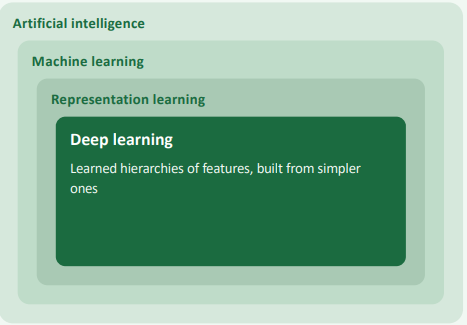
\includegraphics[width=0.7\linewidth]{immagini/where_dl_sits.png} 
    \caption{Hierarchical positioning of Deep Learning }
    \label{fig:where_dl_sits}
\end{figure}

\section{Representation learning}
What really distinguishes deep learning from traditional machine learning is its ability to 
perform \textit{representation learning}. In traditional machine learning, the model is provided with a
set of features that are manually engineered by domain experts. In contrast, deep learning models 
automatically learn to extract relevant features from raw data with representation learning.
In figure \ref{fig:four_approaches} we can see four different approaches to the task of representation.
\begin{figure}[htbp]
    \centering
    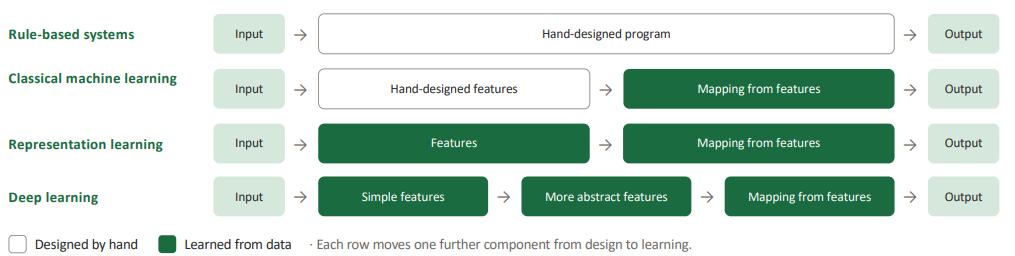
\includegraphics[width=0.85\linewidth]{immagini/four_rep.png} 
    \caption{Four approaches to representation learning}
    \label{fig:four_approaches}
\end{figure}
\noindent
The main goal of representation learning is to identify the \textbf{factor of variations} that explain
the observed data (that sometimes are not directly observable). They might be seen as concepts or 
abstraction that help us make sense of the rich variability in the data.

\section{Deep learning}
Deep learning uses a hierarchical approach to representation learning, allowing models 
to obtain features by introducing representations that are expressed in terms of other 
simpler representations. These architectures frequently leverage \textit{distributed representations},
where concepts are encoded through the joint, many-to-many activity of multiple processing units 
rather than isolated nodes, significantly improving efficiency and generalization.
